\chapter{Prototyping in Office Message System}

\section{System description}
The system involves subscribers, publishers and different topics, as to show the workings of the connext middleware. 

\begin{center}
	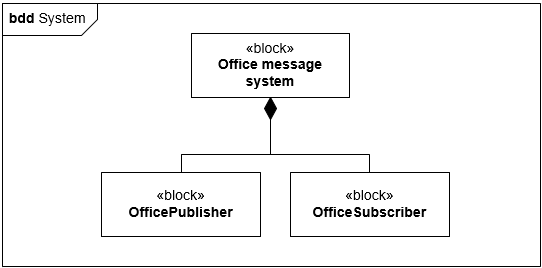
\includegraphics[scale=1.0]{bdd_image.png}
	\captionof{figure}{BDD of the Office Message System}
\end{center}

The office message system is shown in figure 4.1. The system consists of two different classes, the OfficePublisher and the OfficeSubscriber. The specific topic, type and Quality Of Service of the Subscribers/Publishers are determined through constructor injection.

The prototype will consist of two programs running side by side. One will spawn the subscribers and the other will spawn the publishers. All Readers and Writers are configured for sending messages by the string type. 

The configuration is setup as seen in figure 4.2.

\begin{center}
	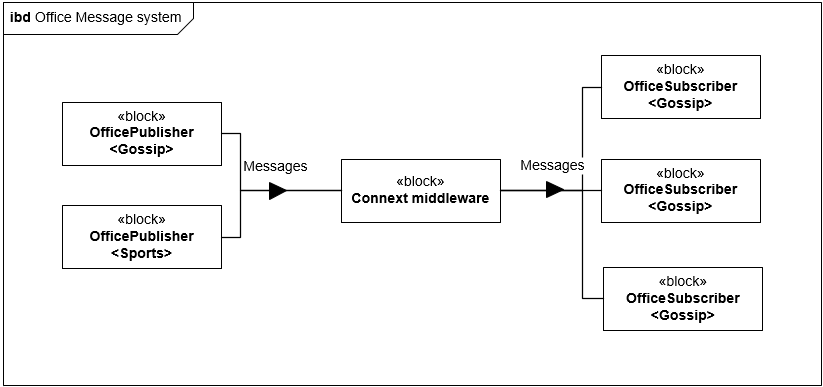
\includegraphics[scale=0.75]{ibd_image.png}
	\captionof{figure}{IBD of the Office Message System}
\end{center}

As is seen, a publisher publishing on the "Gossip" topic and one for the "Sports" topic are in the system. The publishers will communicate to the subscribers through the connext middleware.

\section{Connext RTI}

\subsection{Domain Participant}

\subsection{Topics}


\section{Publisher}
\subsection{DataWriter}

\section{Subscriber}
\subsection{DataReader}


\section{Quality Of Service}


\section{Tests}
